\let\lesson\undefined
\newcommand{\lesson}{\phantomlesson{Bài tập vật lí nhiệt}}
\section{Bài tập trắc nghiệm}
\begin{enumerate}[label=\bfseries Câu \arabic*:, leftmargin=1.7cm]
	\item \mkstar{2}\\
	Một động cơ nhiệt lí tưởng thực hiện một công $\SI{5}{\kilo\joule}$ đồng thời truyền cho nguồn lạnh nhiệt lượng $\SI{15}{\kilo\joule}$. Hiệu suất của động cơ nhiệt này là
	\begin{mcq}(4)
		\item $\SI{33.33}{\percent}$.
		\item $\SI{75}{\percent}$.
		\item $\SI{25}{\percent}$.
		\item $\SI{66.67}{\percent}$.
	\end{mcq}
\hideall{
\textbf{Đáp án C.}\\
$$H=\dfrac{A}{Q_1}=\dfrac{A}{Q_2+A}=\SI{25}{\percent}.$$
}

\item \mkstar{2}\\
Một động cơ nhiệt làm việc giữa hai nguồn nhiệt. Nhiệt lượng tác nhân nhận của nguồn nóng trong một chu trình là $\SI{2400}{\joule}$. Hiệu suất của động cơ nhiệt là $\SI{25}{\percent}$. Nhiệt lượng tác nhân truyền cho nguồn lạnh trong một chu trình là
\begin{mcq}(4)
	\item $\SI{1200}{\joule}$.
	\item $\SI{2400}{\joule}$.
	\item $\SI{600}{\joule}$.
	\item $\SI{1800}{\joule}$.
\end{mcq}
\hideall{
\textbf{Đáp án D.}\\
$$H=1-\dfrac{Q_2}{Q_1}\Rightarrow Q_2=\SI{1800}{\joule}.$$
}

\item \mkstar{2}\\
Một động cơ nhiệt nhả cho nguồn lạnh $\SI{80}{\percent}$ nhiệt lượng mà nó thu được từ nguồn nóng. Hiệu suất của động cơ nhiệt này là
\begin{mcq}(4)
	\item $\SI{20}{\percent}$.
	\item $\SI{37}{\percent}$.
	\item $\SI{50}{\percent}$.
	\item $\SI{80}{\percent}$.
\end{mcq}
\hideall{
\textbf{Đáp án A.}\\
Hiệu suất của động cơ nhiệt:
$$H=1-\dfrac{Q_2}{Q_1}=\SI{20}{\percent}.$$
}


	
	\item \mkstar{2}\\
Người ta phải tốn $\SI{150}{\gram}$ dầu hoả để đun sôi được $\SI{4.5}{\text{lít}}$ nước ở nhiệt độ ban đầu $\SI{20}{\celsius}$. Cho biết khối lượng riêng của nước là $\SI{1}{\kilogram/\text{lít}}$, nhiệt dung riêng của nước là $\SI{4200}{\joule/\left(\kilogram\cdot\kelvin\right)}$, năng suất toả nhiệt của dầu hoả là $\SI{44E6}{\joule/\kilogram}$. Hiệu suất của bếp đun là
\begin{mcq}(4)
	\item $\SI{22.9}{\percent}$.
	\item $\SI{2.29}{\percent}$.
	\item $\SI{12.9}{\percent}$.
	\item $\SI{26.9}{\percent}$.
\end{mcq}
\hideall{
\textbf{Đáp án A.}\\
Hiệu suất của bếp đun:
$$H=\dfrac{m_\text{n}c\Delta t}{m_\text{d}q}=\SI{22.9}{\percent}.$$
}

\item \mkstar{2}\\
Để đun sôi một lượng nước bằng bếp dầu có hiệu suất $\SI{30}{\percent}$, phải dùng hết 1 lít dầu. Để đun sôi cũng lượng nước trên với bếp dầu có hiệu suất $\SI{20}{\percent}$ thì phải dùng
\begin{mcq}(4)
	\item 2 lít dầu.
	\item 0,5 lít dầu.
	\item 1,5 lít dầu.
	\item 3 lít dầu.
\end{mcq}
\hideall{
\textbf{Đáp án C.}\\
$$V_2=\dfrac{V_1H_1}{H_2}=\SI{1.5}{\liter}.$$
}

\item \mkstar{2}\\
Khi dùng lò có hiệu suất $H_1$ để làm chảy một lượng quặng, phải đốt hết $\xsi{m_1}{\left(\kilogram\right)}$ nhiên liệu có năng suất toả nhiệt $q_1$. Nếu dùng lò có hiệu suất $H_2$ để làm chảy lượng quặng trên thì phải đốt hết $m_2=\xsi{3m_1}{\left(\kilogram\right)}$ nhiên liệu có năng suất toả nhiệt $q_2=0,5q_1$. Hệ thức liên hệ giữa $H_1$ và $H_2$ là
\begin{mcq}(4)
	\item $H_1=H_2$.
	\item $H_1=2H_2$.
	\item $H_1=3H_2$.
	\item $H_1=1,5H_2$.
\end{mcq}
\hideall{
\textbf{Đáp án D.}\\
$$H=\dfrac{Q}{mq}$$
$$\Rightarrow \dfrac{H_1}{H_2}=\dfrac{m_2q_2}{m_1q_1}=\dfrac{3}{2}.$$
}

\item \mkstar{3}\\
Một động cơ nhiệt có hiệu suất $\SI{25}{\percent}$ và công suất $\SI{30}{\kilo\watt}$. Nhiệt lượng mà động cơ toả ra cho nguồn lạnh trong 5 giờ làm việc liên tục là
\begin{mcq}(4)
	\item $\SI{176E7}{\joule}$.
	\item $\SI{194E7}{\joule}$.
	\item $\SI{213E7}{\joule}$.
	\item $\SI{162E7}{\joule}$.
\end{mcq}
\hideall{
	\textbf{Đáp án D.}\\
	$$H=\dfrac{A}{A+Q_2}=\dfrac{\calP t}{\calP t+Q_2}\Rightarrow Q_2=\SI{162E7}{\joule}.$$
}

\item \mkstar{3}\\
Một đầu máy diezen xe lửa có công suất $\SI{3E6}{\watt}$ và có hiệu suất $\SI{25}{\percent}$. Cho biết năng suất toả nhiệt của nhiên liệu là $\SI{4.2E7}{\joule/\kilogram}$. Nếu đầu máy chạy hết công suất thì khối lượng nhiên liệu tiêu thụ trong mỗi giờ \textbf{gần giá trị nào nhất} sau đây?
\begin{mcq}(4)
	\item $\SI{2489}{\kilogram}$.
	\item $\SI{1429}{\kilogram}$.
	\item $\SI{1028}{\kilogram}$.
	\item $\SI{1056}{\kilogram}$.
\end{mcq}
\hideall{
\textbf{Đáp án C.}\\
Khối lượng nhiên liệu tiêu thụ trong 1 giờ khi động cơ xe lửa hoạt động hết công suất:
$$m=\dfrac{\calP t}{qH}\approx\SI{1028.57}{\kilogram}.$$

}

\item \mkstar{3}\\
Một máy bơm sau khi tiêu thụ hết $\SI{8}{\kilogram}$ dầu thì đưa được $\SI{700}{\meter^3}$ nước lên cao $\SI{8}{\meter}$. Biết năng suất toả nhiệt của dầu dùng cho  máy bơm này là $\SI{4.6E7}{\joule/\kilogram}$. Xem rằng nước được đưa lên cao một cách đều đặn, khối lượng riêng của nước $\SI{1000}{\kilogram/\meter^3}$, gia tốc trọng trường $g=\SI{10}{\meter/\second^2}$. Hiệu suất của máy bơm là
\begin{mcq}(4)
	\item $\SI{15.22}{\percent}$.
	\item $\SI{24.46}{\percent}$.
	\item $\SI{1.52}{\percent}$.
	\item $\SI{2.45}{\percent}$.
\end{mcq}
\hideall{
\textbf{Đáp án A.}\\
Hiệu suất máy bơm:
$$H=\dfrac{\rho Vgh}{qm_\text{d}}\approx\SI{15.22}{\percent}.$$
}

\item \mkstar{3}\\
Một ô tô chạy $\SI{100}{\kilo\meter}$ với lực kéo không đổi $\SI{700}{\newton}$ thì tiêu thụ hết $\SI{6}{\text{lít}}$ xăng. Biết năng suất toả nhiệt của xăng là $\SI{4.6E7}{\joule/\kilogram}$, khối lượng riêng của xăng là $\SI{700}{\kilogram/\meter^3}$. Hiệu suất của động cơ ô tô là
\begin{mcq}(4)
	\item $\SI{25}{\percent}$.
	\item $\SI{36}{\percent}$.
	\item $\SI{0.36}{\percent}$.
	\item $\SI{17.75}{\percent}$.
\end{mcq}
\hideall{
\textbf{Đáp án B.}\\
Hiệu suất của động cơ ô tô:
$$H=\dfrac{A}{Q}=\dfrac{Fs}{\rho_\text{xăng}Vq}=\SI{36.23}{\percent}.$$
}

\item \mkstar{3}\\
Một nhà máy điện tiêu thụ $\SI{0.35}{\kilogram}$ nhiên liệu cho mỗi $\SI{1}{\kilo\watt\hour}$ điện năng. Cho biết năng suất toả nhiệt của nhiên liệu trên là $\SI{42}{\mega\joule/\kilogram}$. Hiệu suất của động cơ nhiệt dùng trong nhà máy điện \textbf{gần nhất} với giá trị nào sau đây?
\begin{mcq}(4)
	\item $\SI{38}{\percent}$.
	\item $\SI{15}{\percent}$.
	\item $\SI{20}{\percent}$.
	\item $\SI{24}{\percent}$.
\end{mcq}
\hideall{
\textbf{Đáp án .}\\
Hiệu suất của động cơ nhiệt dùng trong nhà máy:
$$H=\dfrac{A}{Q_\text{tp}}=\dfrac{\left(\SI{E3}{\watt}\right)\cdot\left(\SI{3600}{\second}\right)}{\left(\SI{0.35}{\kilogram}\right)\cdot\left(\SI{42E6}{\joule/\kilogram}\right)}\approx\SI{24.5}{\percent}.$$
}

\item \mkstar{3}\\
Một chiếc xe máy hoạt động với công suất $\SI{3.2}{\kilo\watt}$ và chuyển động đều với tốc độ $\SI{45}{\kilo\meter/\hour}$. Hiệu suất của động cơ là $\SI{25}{\percent}$, năng suất toả nhiệt của xăng là $\SI{4.6E7}{\joule/\kilogram}$, khối lượng riêng của xăng là $\SI{700}{\kilogram/\meter^3}$. Với 2 lít xăng thì xe máy đi được bao nhiêu $\si{\kilo\meter}$?
\begin{mcq}(4)
	\item $\SI{100.6}{\kilo\meter}$.
	\item $\SI{63}{\kilo\meter}$.
	\item $\SI{45}{\kilo\meter}$.
	\item $\SI{54}{\kilo\meter}$.
\end{mcq}
\hideall{
\textbf{Đáp án B.}\\
Thời gian động cơ xe máy hoạt động được khi tiêu thụ $\SI{2}{\text{lít}}$ xăng:
$$t=\dfrac{q\rho V}{\calP}\cdot H=\SI{5031.25}{\second}=\SI{1.39}{\hour}.$$
Quãng đường xe máy đi được:
$$s=vt\approx\SI{62.89}{\kilo\meter}.$$
}

\item \mkstar{3}\\
Một động cơ ô tô hoạt động với công suất $\SI{20}{\kilo\watt}$ và ô tô chuyển động đều với tốc độ $\SI{72}{\kilo\meter/\hour}$. Ô tô tiêu thụ $\SI{20}{\text{lít}}$ xăng thì chạy được quãng đường $\SI{200}{\kilo\meter}$. Biết khối lượng riêng của xăng là $\SI{700}{\kilogram/\meter^3}$, năng suất toả nhiệt của xăng là $\SI{4.6E7}{\joule/\kilogram}$. Hiệu suất của động cơ ô tô khi đó là
\begin{mcq}(4)
	\item $\SI{31}{\percent}$.
	\item $\SI{61}{\percent}$.
	\item $\SI{63}{\percent}$.
	\item $\SI{36}{\percent}$.
\end{mcq}
\hideall{
\textbf{Đáp án A.}\\
Hiệu suất của ô tô:
$$H=\dfrac{\calP\cdot\dfrac{s}{v}}{\rho Vq}\approx\SI{31.05}{\percent}.$$
}
	
	\item \mkstar{3}\\
	Dùng một bếp dầu hoả để đun sôi 2 lít nước từ $\SI{15}{\celsius}$ thì mất $\SI{10}{\text{phút}}$. Biết rằng chỉ có $\SI{40}{\percent}$ nhiệt lượng do dầu toả ra làm nóng nước. Lấy nhiệt dung riêng của nước là $\SI{4190}{\joule/\left(\kilogram\cdot\kelvin\right)}$, năng suất toả nhiệt của dầu hoả là $\SI{46E6}{\joule/\kilogram}$, khối lượng riêng của nước là $\SI{1}{\gram/\centi\meter^3}$. Lượng dầu hoả cần dùng trong mỗi phút là
	\begin{mcq}(4)
		\item $\SI{0.619}{\gram}$.
		\item $\SI{0.619}{\kilogram}$.
		\item $\SI{3.87}{\gram}$.
		\item $\SI{3.87}{\kilogram}$.
	\end{mcq}
\hideall{
\textbf{Đáp án C.}\\
Khối lượng dầu cần dùng trong mỗi phút:
$$m=\dfrac{Q}{qH}=\dfrac{mc\Delta t}{qH}=\SI{3.87E-3}{\kilogram}=\SI{3.87}{\gram}.$$
}
	
	\item \mkstar{3}\\
	Người ta cần nấu chảy 10 tấn đồng trong lò nung dùng dầu làm nhiên liệu đốt. Cho biết nhiệt độ ban đầu, nhiệt độ nóng chảy, nhiệt dung riêng và nhiệt nóng chảy riêng của đồng lần lượt là $\SI{13}{\celsius}$, $\SI{1083}{\celsius}$, $\SI{380}{\joule/\left(\kilogram\cdot\kelvin\right)}$, $\SI{1.8E5}{\joule/\kilogram}$. Nhiệt lượng toả ra khi đốt cháy $\SI{1}{\kilogram}$ dầu là $\SI{4.6E7}{\joule/\kilogram}$. Nếu hiệu suất nung của lò là $\SI{30}{\percent}$ thì khối lượng dầu cần dùng là
	\begin{mcq}(4)
		\item $\SI{425.1}{\kilogram}$.
		\item $\SI{127.5}{\kilogram}$.
		\item $\SI{38.3}{\kilogram}$.
		\item $\SI{432.2}{\kilogram}$.
	\end{mcq}
\hideall{
\textbf{Đáp án A.}\\
Nhiệt lượng đồng cần thu vào để nóng chảy hoàn toàn:
$$Q=mc\Delta t+m\lambda=\SI{58.66E8}{\joule}.$$
Khối lượng xăng cần dùng:
$$m=\dfrac{Q}{qH}=\SI{425.1}{\kilogram}.$$
}
	
	\item \mkstar{3}\\
	Một ấm nhôm có khối lượng $m_\text{b}=\SI{600}{\gram}$ chứa $V=\SI{1.5}{\text{lít}}$ nước ở $t_1=\SI{20}{\celsius}$, sau đó đun bằng bếp điện. Sau thời gian $t=\SI{35}{\text{phút}}$ thì đã có $\SI{20}{\percent}$ khối lượng nước đã hoá hơi ở nhiệt độ sôi $t_2=\SI{100}{\percent}$. Biết rằng, $\SI{75}{\percent}$ nhiệt lượng mà bếp cung cấp được dùng vào việc đun nước. Cho biết nhiệt dung riêng của nước là $c_\text{n}=\SI{4190}{\joule/\left(\kilogram\cdot\kelvin\right)}$, của nhôm là $c_\text{b}=\SI{880}{\joule/\left(\kilogram\cdot\kelvin\right)}$, nhiệt hoá hơi riêng của nước ở $\SI{100}{\celsius}$ là $L=\SI{2.26E6}{\joule/\kilogram}$, khối lượng riêng của nước là $D=\SI{1}{\kilogram/\text{lít}}$. Công suất cung cấp nhiệt của bếp điện \textbf{gần giá trị nào nhất} sau đây?
	\begin{mcq}(4)
		\item $\SI{776}{\watt}$.
		\item $\SI{796}{\watt}$.
		\item $\SI{786}{\watt}$.
		\item $\SI{876}{\watt}$.
	\end{mcq}
	\hideall{
		\textbf{Đáp án A.}\\
		Khối lượng nước $$m_\text{n}=VD=\SI{1.5}{\kilogram}.$$
		Tổng nhiệt lượng nước và ấm thu vào:
		$$Q=\left(m_\text{n}c_\text{n}+m_\text{b}c_\text{b}\right)\cdot\left(t_2-t_1\right)+\SI{20}{\percent}m_\text{n}L=\SI{1223040}{\joule}.$$
		Điện năng tiêu thụ của ấm:
		$$A=\dfrac{Q}{H}=\SI{1630720}{\joule}.$$
		Công suất của ấm điện:
		$$\calP=\dfrac{A}{t}\approx\SI{776.5}{\watt}.$$	
	}
\end{enumerate}

\section{Trắc nghiệm đúng/sai}
\begin{enumerate}[label=\bfseries Câu \arabic*:, leftmargin=1.7cm]
	\item \mkstar{2}\\
	Cầu chì là linh kiện được sử dụng để bảo vệ thiết bị và lưới điện tránh sự cố ngắn mạch, hạn chế tình trạng cháy, nổ.
	\begin{center}
		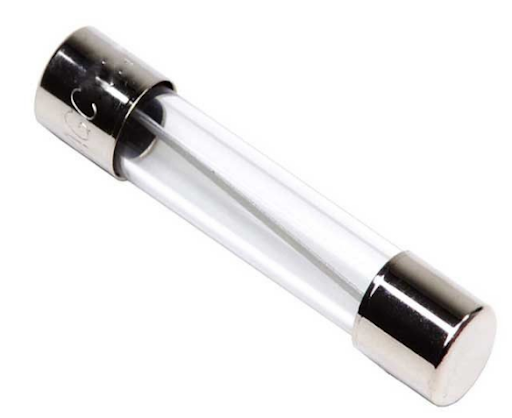
\includegraphics[width=0.25\linewidth]{../figs/VN12-Y24-PH-SYL-007P-1}
	\end{center}
	\begin{enumerate}[label=\alph*)]
		\item Cầu chì có thể bảo vệ mạch điện dựa trên sự phụ thuộc của điện trở kim loại theo nhiệt độ.
		\item Dây chảy trong cầu chì thường được làm từ kim loại có nhiệt độ nóng chảy cao.
		\item Khi cường độ dòng điện qua mạch tăng vượt hạn, dây chì sẽ nóng chảy trước.
		\item Khi dây chảy trong cầu chì bị đứt, ta có thể nối cầu chì bằng dây sắt.
	\end{enumerate}
\hideall{
\begin{enumerate}[label=\alph*)]
	\item Sai. Khi dòng điện qua mạch vượt hạn, dây chảy trong cầu chì nóng chảy trước và là hở mạch.
	\item Sai. Dây chảy được làm từ kim loại có nhiệt độ nóng chảy thấp.
	\item Đúng.
	\item Sai. Sắt là kim loại có nhiệt độ nóng chảy cao, khi cường độ dòng điện tăng quá lớn nhưng dây sắt nóng chảy chậm nên không bảo vệ được mạch điện.
\end{enumerate}
}
\end{enumerate}
\section{Bài tập tự luận}
\begin{enumerate}[label=\bfseries Câu \arabic*:, leftmargin=1.7cm]
	\item \mkstar{2}\\
	Một bếp dầu đun sôi 1 lít nước đựng trong ấm bằng nhôm khối lượng $m_2=\SI{300}{\gram}$ thì sau thời gian $t_1=\SI{10}{\minute}$ nước sôi. Nếu dùng bếp trên để đun 2 lít nước trong cùng điều kiện thì sau bao lâu nước sôi? Cho nhiệt dung riêng của nước và nhôm lần lượt là $c_1=\SI{4200}{\joule/\left(\kilogram\cdot\kelvin\right)}$, $c_2=\SI{880}{\joule/\left(\kilogram\cdot\kelvin\right)}$. Biết nhiệt do bếp dầu cung cấp một cách đều đặn.
	\hideall{
Vì bếp dầu cung cấp nhiệt lượng một cách đều đặn nên
$$\dfrac{t_2}{t_1}=\dfrac{\left(m_2c_2+m'_1c_1\right)\Delta t}{\left(m_2c_2+m_1c_1\right)\Delta t}=\dfrac{m_2c_2+m'_1c_1}{m_2c_2+m_1c_1}\Rightarrow t_2\approx\SI{19.4}{\minute}.$$
}
	
\item	\mkstar{3}\\
Khi thả một quả cầu nhôm khối lượng $\SI{500}{\gram}$ vào $\SI{2}{\kilogram}$ nước ở $\SI{25}{\celsius}$ thì nhiệt độ của chúng sau khi cân bằng nhiệt là $\SI{30}{\celsius}$. Hỏi nhiệt độ ban đầu của quả cầu nhôm là bao nhiêu? Biết nhiệt lượng hao phí trong trường hợp này bằng $\SI{20}{\percent}$ nhiệt lượng do nước thu vào. Biết nhiệt dung riêng của nhôm là $\SI{880}{\joule/\left(\kilogram\cdot\kelvin\right)}$, nhiệt dung riêng của nước là $\SI{4200}{\joule/\left(\kilogram\cdot\kelvin\right)}$. Bỏ qua sự hoá hơi của nước ngay khi tiếp xúc với quả cầu.
	\hideall{
		Khi hệ cân bằng nhiệt, tổng nhiệt lượng trao đổi trong hệ bằng 0:
		\begin{eqnarray*}
			&&Q_1+Q_2+Q_\text{hp}=0\\
			&\Leftrightarrow& m_1C_1\left(t_\text{cb}-t_1\right)+1,2m_2C_2\left(t_\text{cb}-t_2\right)=0\\
			&\Rightarrow& t_1\approx\SI{144.55}{\celsius}.
		\end{eqnarray*}
	}

\item \mkstar{3}\\
Động cơ nhiệt lí tưởng làm việc giữa hai nguồn nhiệt $\SI{27}{\celsius}$ và $\SI{127}{\celsius}$. Nhiệt lượng tác nhân nhận từ nguồn nóng trong một chu trình là $\SI{2400}{\joule}$. Tính:
\begin{enumerate}[label=\alph*)]
	\item hiệu suất của động cơ.
	\item công thực hiện trong một chu trình.
	\item nhiệt lượng truyền cho nguồn lạnh trong một chu trình.
\end{enumerate}
\hideall{
\begin{enumerate}[label=\alph*)]
	\item $H=\dfrac{T_1-T_2}{T_1}=\SI{25}{\percent}.$
	\item $A=H\cdot Q_1=\SI{600}{\joule}$.
	\item $Q_2=Q_1-A=\SI{1800}{\joule}$.
\end{enumerate}
}

\item \mkstar{3}\\
Máy hơi nước công suất $\SI{1}{\kilo\watt}$ tiêu thụ $\SI{10}{\kilogram}$ than đá trong 1 giờ. Biết hơi nước vào và ra cylanh có nhiệt độ $\SI{227}{\celsius}$ và $\SI{100}{\celsius}$. Năng suất toả nhiệt của than đá là $\SI{3.6E7}{\joule/\kilogram}$. Tính hiệu suất thực của máy và của một động cơ nhiệt lý tưởng làm việc giữa hai nhiệt độ nói trên.
\hideall{
Hiệu suất của máy:
$$H=\dfrac{A}{Q}=\dfrac{\calP t}{mq}=\SI{10}{\percent}.$$
Hiệu suất của động cơ nhiệt lí tưởng:
$$H_\text{max}=\dfrac{T_1-T_2}{T_1}=\SI{25.4}{\percent}.$$
}

\item \mkstar{3}\\
Một động cơ hơi nước lí tưởng là động cơ nhiệt có hiệu suất cực đại, hoạt động với nguồn nóng là lò hơi có nhiệt độ $\SI{500}{\kelvin}$. Nước được đưa vào lò hơi và được đun nóng để chuyển thể thành hơi nước. Hơi nước này làm piston chuyển động. Nhiệt độ của nguồn lạnh là nhiệt độ bên ngoài của không khí, bằng $\SI{300}{\kelvin}$.
\begin{enumerate}[label=\alph*)]
	\item Tính công của động cơ hơi nước thực hiện khi lò hơi cung cấp cho tác nhân một nhiệt lượng bằng $\SI{6.5E3}{\joule}$.
	\item Giả sử muốn tăng hiệu suất này lên $\SI{45}{\percent}$ phải tăng nhiệt độ lò hơi lên một lượng bằng bao nhiêu?
\end{enumerate}
\hideall{
\begin{enumerate}[label=\alph*)]
	\item $H=\dfrac{A}{Q_1}=\dfrac{T_1-T_2}{T_1}\Rightarrow A=\SI{2600}{\joule}$.
	\item $H_\text{max}=\dfrac{T_1-T_2}{T_1}\Rightarrow T_1\approx\SI{545.46}{\kelvin}.$
\end{enumerate}
}

\item \mkstar{3}\\
Búa máy 10 tấn rơi từ độ cao $\SI{2.3}{\meter}$ xuống một cọc sắt khối lượng $\SI{200}
{\kilogram}$. Biết $\SI{40}{\percent}$ động năng của búa biến thành nhiệt làm nóng cọc sắt. Hỏi búa rơi bao nhiêu lần thì cọc tăng nhiệt độ thêm $\SI{20}{\celsius}$. Cho rằng cọc không toả nhiệt ra môi trường và nhiệt dung riêng của sắt là $\SI{0.46}{\kilo\joule/\left(\kilogram\cdot\kelvin\right)}$.
\hideall{
\begin{itemize}
	\item Động năng của búa ngay trước khi va chạm với cọc: $W_\text{đ}=Mgh$.
	\item Nhiệt lượng cọc thu được sau mỗi lần búa rơi: $Q_0=0,4W_\text{đ}=0,4Mgh$.
	\item Nhiệt lượng cọc thu được sau $n$ lần búa rơi: $Q=nQ_0=mc\Delta t$.
\end{itemize}
Suy ra:
$$n=\dfrac{mc\Delta t}{0,4Mgh}=20.$$
}
\end{enumerate}
